% 
% Annual Cognitive Science Conference
% Sample LaTeX Paper -- Proceedings Format
% 

% Original : Ashwin Ram (ashwin@cc.gatech.edu)       04/01/1994
% Modified : Johanna Moore (jmoore@cs.pitt.edu)      03/17/1995
% Modified : David Noelle (noelle@ucsd.edu)          03/15/1996
% Modified : Pat Langley (langley@cs.stanford.edu)   01/26/1997
% Latex2e corrections by Ramin Charles Nakisa        01/28/1997 
% Modified : Tina Eliassi-Rad (eliassi@cs.wisc.edu)  01/31/1998
% Modified : Trisha Yannuzzi (trisha@ircs.upenn.edu) 12/28/1999 (in process)
% Modified : Mary Ellen Foster (M.E.Foster@ed.ac.uk) 12/11/2000
% Modified : Ken Forbus                              01/23/2004
% Modified : Eli M. Silk (esilk@pitt.edu)            05/24/2005
% Modified : Niels Taatgen (taatgen@cmu.edu)         10/24/2006
% Modified : David Noelle (dnoelle@ucmerced.edu)     11/19/2014

%% Change "letterpaper" in the following line to "a4paper" if you must.

\documentclass[10pt,letterpaper]{article}

\usepackage{cogsci}
\usepackage{pslatex}
\usepackage[natbibapa]{apacite}
\usepackage{amsmath}
\usepackage{amssymb}
\usepackage{dsfont}
\usepackage{xcolor}

\newcommand{\fl}[1]{\textcolor{red}{\textsc{[#1 -Falk]}}}
\newcommand{\pd}[1]{\textcolor{blue}{\textsc{[#1 -Priyam]}}}
\newcommand{\sg}[1]{\textcolor{purple}{\textsc{[#1 -Sayan]}}}
\newcommand{\tlg}[1]{\textcolor{magenta}{\textsc{[#1 -Paul]}}}
\newcommand{\fc}[1]{\textcolor{green}{\textsc{[#1 -Fred]}}}


\title{Bounded optimality predicts human planning strategies}
%Discovering planning strategies by resource-rational analysis
 
\author{
  {\large \bf TBD}
  %Morton Ann Gernsbacher (MAG@Macc.Wisc.Edu)} \\
  %Department of Psychology\\
  %UC Berkeley
  \AND {\large \bf TBD} 
  }


\begin{document}

\maketitle
\fl{Fred's original title was ``Heuristic planning strategies as resource-rational metareasoning'' but I don't want to claim that people choose their computations through explicit meta-reasoning. I also don't think we are ready to make a statement about the resource-rationality of the metareasoning process itself. At best we can say something about the resulting strategies. Another option for our title is ``Discovering planning strategies by resource-rational analysis''.}

\begin{abstract}
Abstract

\textbf{Keywords:} 

\end{abstract}




\section{Introduction}
\label{sec:introduction}

% Bounded optimality & planning strategies
% Introduce the method for discovering cognitive strategies
% Application to planning strategies


\section{Mouselab MDP}
\label{sec:mouselab_mdp}

% Shortened version of RLDM paper introducing mouselab-MDP
%\fl{TODO: Fred and Falk, Paul and Sayan can help too}
Planning, like all of cognition, is a mental process that cannot be observed directly. Thus, to compare people's planning strategy to the bounded-optimal planning strategy, we first had to make it observable. To do so, we developed a process tracing paradigm for the study of planning \cite{CallawayLiederKrueger2017}. Our Mouselab-MDP paradigm is inspired by the Mouselab paradigm \citep{Payne1993} that traces how people choose between multiple risky gambles. The basic idea is to externalize people's mental simulations of alternative action sequences. To do so, the Mouselab-MDP paradigm presents participants with a route planning problem where each move earns or loses an initially unknown amount of money. The participant's goal is to choose a route in such a way that they earn as much money as possible. To find out how much money a transition would yield the participant has to click on it and pay a fee. Each click is recorded and the recorded sequence of clicks reveals which paths participants mentally simulated and in which order. This is because finding out the payoff for a simulated move requires clicking on it. Figure \ref{fig:MouselabMDP} illustrates the Mouselab-MDP paradigm with the task used to teach people how to plan better.

\begin{figure}
    \centering
    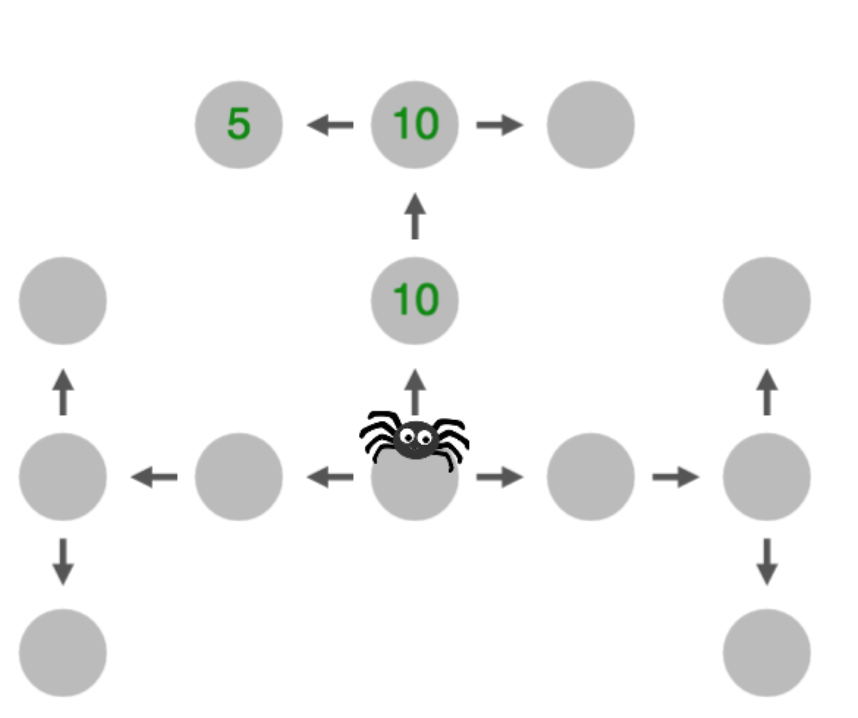
\includegraphics[width=0.4\textwidth]{figures/web-of-cash.png}
    \label{fig:MouselabMDP}
    \caption{Illustration of the Mouselab-MDP paradigm.}
\end{figure}

\newcommand{\A}{\mathcal{A}}
\newcommand{\B}{\mathcal{B}}
\newcommand{\T}{\mathcal{T}}
\newcommand{\meta}{_{\text{meta}}}
\newcommand{\Qmeta}{$Q\meta ^\star$}
\newcommand{\expect}[1]{\mathds{E} \left[ #1 \right]}

\section{Bounded-Optimal planning in the Mouselab-MDP paradigm}
\label{sec:mouselab_mdp}

%\fl{Here we define bounded-optimal planning in Mouselab-MDP paradigm as the solution to a meta-level MDP. We then say that we solve that meta-level MDP with our strategy-discovery method without going into details.}

Following the strategy discovery method developed by \cite{LiederCallawayGulKruegerGriffiths2017}, we model the problem of deciding how to plan as a meta-level Markov decision process (meta-level MDP) \cite{Hay2012}.
Concretely, we model the optimal planning strategy for the Mouselab-MDP paradigm as the solution to the meta-level MDP
\begin{equation}
    M\meta = (\B, \A, \T, r\meta),\label{eq:MouselabMDPMetaMDP}
\end{equation}
where each belief state $b$ encodes one Normal distribution for each transition's reward. Thus, the belief state $b^{(t)}$ at time $t$ can be represented as $((\mu_1^{(t)},\sigma_1^{(t)}), \cdots, (\mu_K^{(t)},\sigma_K^{(t)}))$ such that $b^{(t)}(\theta_k=x)=\mathcal{N}(x; \mu_k^{(t)}, {\sigma_k^{(t)}}^2)$.
The initial belief state $b^{(0)}$ encodes the joint distribution $\mathcal{N}(\mathbf{x}; (\mu^{(R)}_1,\cdots,\mu^{(R)}_K), \Sigma^{(R)}$ the rewards are sampled from. 
The metalevel actions are $\A = \{c_1, \cdots, c_K, \bot\}$ where $c_k$ reveals the reward at state $k$ and $\bot$ selects the path with highest expected sum of rewards according to the current belief state.
The transition probabilities $T\meta(b^{(t)}, c_k, b^{(t+1)})$ encode that performing computation $c_k$ sets $(\mu_k^{(t+1)}, \sigma_k^{(t+1)})$ to $(x,0)$ with probability density $\phi(x;\mu_k^{(t)},\sigma_k^{(t)})$ where $\phi$ is the density function of the normal distribution.
The metalevel reward function is $r\meta(b, c) = -\lambda$ for $c \in \{c_1,\cdots, c_K \}$, and $r\meta\left( (\mu_1,\sigma_1),\cdots, (\mu_K,\sigma_K)), \bot\right) = \max_{\mathbf{t}\in \mathcal{T}} \sum_{k \in \mathbf{t}} \mu_k$ where $\mathcal{T}$ is the set of possible trajectories $\mathbf{t}$ through the environment.



Having formulated the problem of deciding how to plan in these terms, we can now compute the optimal planning strategy by solving the meta-level MDP using dynamic programming \cite{Puterman2014}.\fl{TODO: Fred, is this accurate enough, or is there a simple way to describe your exact solution more accurately?}
%applying the meta-level reinforcement learning method developed by \cite{LiederCallawayGulKruegerGriffiths2017}.

\fl{This is technical,but I think without it bounded optimal planning would be left undefined.}


\section{Experiments}
\label{sec:experiments}

% For each experiment
%   Describe experiment-unique structure
%   Derive qualitative predictions
%   Results
%   Qualitative predictions
%   Quantitative model comparisons

% Experiment 1: effect of increasing vs. decreasing variance
% Experiment 2: effect of low vs. high variance
% Experiment 3: branching and depth


\section{Conclusion}
\label{sec:conclusion}

\paragraph{Summary and Interpretation of the results}
\fl{TODO: Fred, Priyam, Falk, Paul, and Sayan}

\paragraph{Implications and future directions}
\fl{TODO: Falk and Fred}

\bibliographystyle{apacite}

\setlength{\bibleftmargin}{.125in}
\setlength{\bibindent}{-\bibleftmargin}

\bibliography{references}


\end{document}
